%% Supplementary Information for the ver3 manuscript (main_v3.tex). English version of ja_v3/11_補足資料.md (2026-11-17 night).
\documentclass[sn-nature,pdflatex]{sn-jnl}
\usepackage{amsmath,amssymb,amsfonts}
\usepackage{graphicx}
\usepackage{booktabs}
\usepackage{multirow}
\usepackage{xcolor}
\usepackage{array}
\newcommand{\pt}{\,points}
\renewcommand{\thesection}{S\arabic{section}}
\renewcommand{\thetable}{S\arabic{table}}
\renewcommand{\thefigure}{S\arabic{figure}}
\begin{document}
\title{Supplementary Information: Multimodal emotion recognition on a new corpus with a few labels}
\author{TODO}
\maketitle

\section{Can audio features predict the text classifier's decisions?}\label{sec:s1}
As one candidate reason for the audio gains in Sect. 5 of the main text, we examined whether audio features can predict the text classifier's decisions contained in the product.

\subsection{Setting}
As one candidate reason for the audio gains, we examine the explanation that speech carries both voice quality and the spoken words: the product contains the text classifier's decisions, so if audio features can predict those decisions, the audio classifier can learn that part from the pseudo-labels. The cross-modal predictability $D$ is measured as follows: the decisions $J$ of one modality's K-label baseline (e.g., text) are the target; a linear classifier on another modality's features (e.g., audio) predicts $J$ out of sample, and its UAR with $J$ as truth is $R$; the same is done after permuting $J$ within strata of true emotion and speaker cluster (and gender for IEMOCAP and AFEW), giving $R'$; and $D=R-R'$ is the agreement not explained by emotion and speaker. The decision rule was fixed at K = 5 before computing, and AFEW, whose text is a transcript of its own audio, was excluded from the audio--text comparison. We also rebuilt the last-layer WavLM-large features of time-reversed speech of IEMOCAP (improvised), MOSEI and MELD and measured the same $D$ (predictions and rules fixed before computing; the question was set after seeing the non-reversed results). On reversed speech, Whisper large-v3 transcripts agreed with the original words only 0.005--0.012 above chance (0.79--0.80 for the original speech).



\subsection{Results: audio features predicted the text classifier's decisions better than visual features}
On the three corpora other than AFEW, the predictability $D$ of the text classifier's decisions was 19.3 (IEMOCAP), 10.5 (MOSEI) and 17.7 (MELD) points with audio features and 2.0, 0.3 and 3.8 with visual features; the differences (+17.3, +10.2, +13.9) all had intervals above zero. Audio features did not meet the pre-set rule at K = 5 for predicting the visual classifier's decisions better than text features. $D$ may also include agreement from arousal, speaker attributes, utterance duration and recording conditions. Reversing the speech lowered $D$ to 10.5, 3.1 and 10.5 (differences 8.8 [3.0, 14.7], 7.5 [6.3, 8.6] and 7.2 [4.7, 9.8]) (Fig.~\ref{fig:reverse}), but reversed audio still exceeded visual features (by 8.5 [3.8, 13.1], 2.7 [1.3, 4.1] and 6.7 [3.8, 9.6]). Audio's prediction of the text classifier's decisions was therefore not explained by intelligible words alone; the remainder may come from the average spectrum, the pitch distribution, utterance duration, intensity differences within an emotion label or word information left in WavLM features, which this experiment cannot separate.

\begin{figure}[t]
\centering
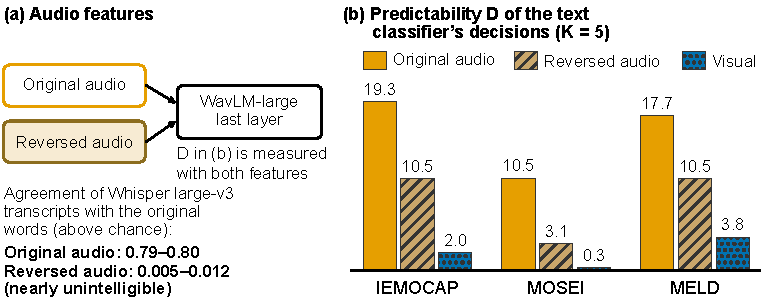
\includegraphics[width=\textwidth]{figures/fig_reverse_en.pdf}
\caption{Predictability $D$ of the text classifier's decisions at K = 5 (UAR points) by original audio, time-reversed audio (words nearly unintelligible) and visual features. The visual value is the reversed-audio $D$ minus the measured difference (reversed audio $-$ visual). AFEW is excluded because its text is a transcript of its own audio}\label{fig:reverse}
\end{figure}


\textbf{Limitation.} Reversed speech was checked with Whisper transcripts, not with human listeners. Reversal also inverts time-directional cues such as intonation contours and produces speech unlike the data WavLM was trained on, so the drop in $D$ should not be attributed to intelligible words alone; measuring $D$ with another manipulation that makes words unintelligible is the next step.

\section{Further comparisons for RQ2}\label{sec:s2}
\subsection{Comparators fitted on the K labels}
\begin{table}[h]
\caption{UAR of the three comparators fitted on the K labels (points, test utterances, mean of 50 repetitions; moved from Table 8 of the main text). Parentheses: estimation-time proposal $-$ row with 95\% intervals without correction; * interval above zero, $\dagger$ below zero. Intervals of the weight-table search are conditional on the drawn tables. Strength-only weights gave the same UAR as the proposal without profiles (Table 9 of the main text) in 8 of the 12 conditions on the four corpora and in all three on CREMA-D}\label{tab:s1}
\footnotesize\setlength{\tabcolsep}{2pt}
\begin{tabular}{@{}llll@{}}
\toprule
Row & K = 5 & K = 10 & K = 25 \\
\midrule
\multicolumn{4}{@{}l}{\textbf{AFEW}} \\
Strength only & 72.51 ($-$1.16 [$-$2.6, +0.3]) & 73.94 (+0.45 [$-$0.1, +1.0]) & 76.55 (+0.03 [$-$0.5, +0.6]) \\
Full table (K) & 72.55 ($-$1.19 [$-$2.8, +0.4]) & 74.34 (+0.05 [$-$0.6, +0.7]) & 76.84 ($-$0.26 [$-$0.8, +0.3]) \\
Table search & 71.50 ($-$0.14 [$-$2.4, +2.1]) & 73.80 (+0.59 [$-$1.2, +2.3]) & 76.55 (+0.03 [$-$1.9, +1.9]) \\
\multicolumn{4}{@{}l}{\textbf{IEMOCAP (improvised)}} \\
Strength only & 72.32 (+0.24 [+0.03, +0.5]*) & 73.57 (+0.23 [$-$0.05, +0.5]) & 74.83 (+0.20 [$-$0.1, +0.5]) \\
Full table (K) & 72.36 (+0.20 [$-$1.7, +2.1]) & 73.75 (+0.05 [$-$0.7, +0.8]) & 75.30 ($-$0.27 [$-$1.1, +0.5]) \\
Table search & 70.41 (+2.15 [+0.9, +3.4]*) & 71.30 (+2.50 [+1.7, +3.3]*) & 73.49 (+1.54 [+1.2, +1.9]*) \\
\multicolumn{4}{@{}l}{\textbf{MOSEI}} \\
Strength only & 40.43 (+0.73 [+0.5, +1.0]*) & 42.20 (+0.62 [+0.4, +0.9]*) & 43.96 (+0.51 [+0.3, +0.8]*) \\
Full table (K) & 40.62 (+0.54 [$-$0.01, +1.1]) & 42.31 (+0.51 [+0.1, +0.9]*) & 44.08 (+0.39 [+0.1, +0.7]*) \\
Table search & 40.06 (+1.10 [+0.6, +1.6]*) & 41.48 (+1.34 [+0.9, +1.8]*) & 42.80 (+1.66 [+1.2, +2.1]*) \\
\multicolumn{4}{@{}l}{\textbf{MELD}} \\
Strength only & 50.52 ($-$0.46 [$-$1.3, +0.3]) & 50.89 ($-$0.20 [$-$1.0, +0.6]) & 52.80 (+0.15 [$-$0.1, +0.4]) \\
Full table (K) & 49.37 (+0.68 [$-$0.2, +1.5]) & 50.39 (+0.29 [$-$0.4, +1.0]) & 52.53 (+0.42 [$-$0.02, +0.9]) \\
Table search & 49.47 (+0.59 [$-$0.5, +1.7]) & 49.67 (+1.01 [+0.1, +2.0]*) & 51.47 (+1.48 [+0.7, +2.3]*) \\
\botrule
\end{tabular}
\end{table}


\subsection{Four further combinations of the same predictions}
Table~\ref{tab:extra} compares the estimation-time proposal with four further combinations of the predictions of the same product components, computed in the same evaluation run as Table 8 of the main text; the proposal and each combination use the label-free intercept shift of Sect. 6.1.2 of the main text. \emph{Exponents from other corpora} multiplies the three probabilities raised to one exponent per modality (common to emotions), chosen on provisional targets in Sect. 5.1.1 of the main text and normalised to mean 1; on AFEW the selected exponents were (1, 1, 1), so its decisions equal those of the product. \emph{Confidence-weighted mean} averages the three probabilities, each weighted per utterance by the classifier's maximum probability (a confidence-weighted late fusion used as a baseline by Tellamekala et al.\ \cite{tellamekala2024}; using the maximum probability as the confidence is our choice). \emph{Table re-reading} re-reads each classifier's probabilities with a diagonal confusion table measured on the K labels (off-diagonal entries $(1-\text{diagonal})/3$), shrunk halfway towards a table with the classifier's mean diagonal, and multiplies them; classifiers whose mean diagonal is at most 0.25 are not used. \emph{Modality weights from K} fits three modality weights (common to emotions) jointly to the log-likelihood of the combined prediction on the K labels (a weighted log-linear pool \cite{heskes1997}).

\begin{table}[h]
\caption{Estimation-time proposal $-$ further combinations (UAR points, test utterances, mean of 50 repetitions) with 95\% intervals without correction. * interval above zero (proposal higher); $\dagger$ below zero. IEMOCAP: improvised part}\label{tab:extra}
\footnotesize\setlength{\tabcolsep}{3pt}
\begin{tabular}{@{}llll@{}}
\toprule
Corpus & K = 5 & K = 10 & K = 25 \\
\midrule
\multicolumn{4}{@{}l}{\textit{Exponents from other corpora}} \\
AFEW & +2.13 [+1.0, +3.3]* & +3.51 [+1.5, +5.5]* & +3.14 [+1.9, +4.4]* \\
IEMOCAP & +2.52 [+0.4, +4.6]* & +2.36 [+0.6, +4.1]* & +2.72 [+1.4, +4.0]* \\
MOSEI & +0.45 [$-$0.02, +0.9] & +0.49 [+0.04, +0.9]* & +0.57 [+0.1, +1.0]* \\
MELD & +2.10 [+0.5, +3.7]* & +2.42 [+1.5, +3.3]* & +2.94 [+1.7, +4.2]* \\
\multicolumn{4}{@{}l}{\textit{Confidence-weighted mean}} \\
AFEW & +2.07 [+0.7, +3.5]* & +3.23 [+1.7, +4.8]* & +3.31 [+1.8, +4.8]* \\
IEMOCAP & +0.07 [$-$1.5, +1.6] & +0.11 [$-$2.2, +2.4] & +0.14 [$-$2.1, +2.3] \\
MOSEI & +0.24 [$-$0.2, +0.6] & +0.33 [$-$0.1, +0.7] & +0.71 [+0.4, +1.1]* \\
MELD & +0.01 [$-$1.3, +1.3] & +0.45 [$-$0.4, +1.3] & +0.93 [+0.2, +1.7]* \\
\multicolumn{4}{@{}l}{\textit{Table re-reading}} \\
AFEW & $-$0.63 [$-$1.9, +0.6] & +0.71 [$-$0.2, +1.6] & +0.29 [$-$0.8, +1.4] \\
IEMOCAP & $-$0.39 [$-$2.6, +1.8] & $-$0.48 [$-$2.3, +1.4] & $-$0.82 [$-$3.1, +1.5] \\
MOSEI & +1.98 [+1.1, +2.9]* & +1.18 [+0.6, +1.7]* & +1.08 [+0.6, +1.6]* \\
MELD & +1.10 [$-$0.2, +2.3] & +0.39 [$-$0.7, +1.5] & +0.21 [$-$0.5, +1.0] \\
\multicolumn{4}{@{}l}{\textit{Modality weights from K}} \\
AFEW & $-$3.54 [$-$8.0, +0.9] & $-$1.57 [$-$4.8, +1.6] & $-$1.50 [$-$3.8, +0.8] \\
IEMOCAP & +2.30 [+0.6, +4.0]* & +1.38 [+0.4, +2.3]* & +0.90 [+0.5, +1.3]* \\
MOSEI & +2.30 [+1.6, +3.0]* & +1.61 [+1.0, +2.2]* & +0.90 [+0.4, +1.4]* \\
MELD & +0.57 [$-$0.6, +1.8] & $-$0.15 [$-$1.4, +1.1] & $-$0.08 [$-$0.7, +0.6] \\
\botrule
\end{tabular}
\end{table}



\section{CREMA-D}\label{sec:s3}
CREMA-D was added to the evaluation after its values had been seen in six-corpus provisional-target computations (Sect. 6.1.3 of the main text). Estimation-time proposal $-$ product and retrained AV proposal $-$ distillation (product) were +0.31 to +0.63\pt\ with all six intervals excluding zero.

\begin{table}[h]
\caption{CREMA-D (audio and visual): UAR (points, test utterances, mean of 50 repetitions; moved from Table 8 of the main text). Rows and marks as in Table 8; the retrained classifier is AV. The strongest single classifier was not computed for CREMA-D}\label{tab:s3}
\footnotesize\setlength{\tabcolsep}{2pt}
\begin{tabular}{@{}llll@{}}
\toprule
Row & K = 5 & K = 10 & K = 25 \\
\midrule
Proposal (est.) & 85.48 & 86.17 & 87.70 \\
Product & 85.01 (+0.47 [+0.2, +0.8]*) & 85.54 (+0.63 [+0.3, +0.9]*) & 87.13 (+0.57 [+0.3, +0.9]*) \\
Mean of probs. & 84.70 (+0.78 [+0.4, +1.2]*) & 85.23 (+0.94 [+0.5, +1.4]*) & 86.92 (+0.77 [+0.3, +1.2]*) \\
Strength only & 85.26 (+0.23 [+0.1, +0.4]*) & 85.89 (+0.27 [+0.1, +0.4]*) & 87.46 (+0.23 [+0.05, +0.4]*) \\
Full table (K) & 85.19 (+0.29 [$-$0.01, +0.6]) & 86.05 (+0.11 [$-$0.1, +0.4]) & 87.71 ($-$0.01 [$-$0.2, +0.2]) \\
Temperature & 85.26 (+0.22 [$-$0.1, +0.5]) & 86.04 (+0.12 [$-$0.1, +0.4]) & 87.55 (+0.14 [$-$0.1, +0.4]) \\
Table search & 84.24 (+1.24 [+0.5, +2.0]*) & 85.46 (+0.71 [+0.1, +1.3]*) & 86.75 (+0.94 [+0.5, +1.4]*) \\
Proposal (retr.) & 85.64 & 86.53 & 87.74 \\
K-label base. & 82.34 (+3.30 [+2.6, +4.0]*) & 83.35 (+3.18 [+2.5, +3.8]*) & 85.34 (+2.40 [+1.9, +2.9]*) \\
Distill. (prod.) & 85.32 (+0.31 [+0.1, +0.6]*) & 86.01 (+0.52 [+0.3, +0.8]*) & 87.35 (+0.39 [+0.1, +0.7]*) \\

\botrule
\end{tabular}
\end{table}

\section{Other loss forms for retraining on pseudo-labels}\label{sec:s4}
The main loss (form (a), without temperature) was fixed before the evaluation run. For comparison, five other loss forms that take the pseudo-labels were trained in the same way, and for each target, classifier and K the form with the highest provisional-target UAR was compared with form (a): a temperature loss (form (b)) \cite{hinton2015distilling} with $\tau=2$ from Albanie et al.\ \cite{albanie2018}, pseudo-labels on agreeing utterances only \cite{shi2024audioguided}, mixing with the classifier's own predictions \cite{zhang2021combining}, soft co-training (our variant of the idea of \cite{blum1998}) and co-regularisation \cite{sindhwani2005coreg}; each adapts the loss of the original paper to take the pseudo-labels as targets and is not identical to the original method. Replacing form (a) by the form selected on provisional targets (form (b) in all 16 audio conditions with K = 0, 5, 10, 25) changed audio UAR by $-$0.79 to +0.87\pt, and the selected hyperparameters gave the same classifier as the untuned values in all 16 audio conditions. These results suggest that the audio gains did not come from the choice of loss form or of hyperparameters.

\bibliography{references}
\end{document}
